% !TeX root = ../document_maitre.tex

La première technologie d'\gls{IA} envisagée dans le logiciel SkinSoft est le \gls{NLP} au sens large. L'objectif est d'améliorer l'accessibilité aux données stockées ainsi que l'usage de l'application par le langage naturel.  Ce dernier permet à l'utilisateur de contextualiser sa demande à la de phrase, augmentant la compréhension du besoin utilisateur. Ainsi, un besoin utilisateur mieux exprimer et mieux compris permettrais d'apporter des solutions et reponses de meilleure qualités. Permettre l'interaction en langage naturel entre l'utilisateur et l'application ouvre la voie à deux axes : l'amélioration du système de recherche dans les données, et l'amélioration de la compréhension et de l'utilisation de l'application. 

Avant de développer les deux axes, auxquels le \gls{NLP} répond au travers d'outils et processus différents, il est fondamental de comprendre le fonctionnement d'origine de l'application. Cette partie est donc consacré à l'exploration de la manière dont le logiciel SkinSoft fonctionne sur les deux axes dépeind. Ainsi, nous pourrons mettre en évidences les limites actuelles auxquelles l'intégration du \gls{NLP} doit répondre.\newline

Le stockage et la recherche des données sont fondamentale pour un \terme{SGC}. David Bearman sépare deux éléments, le \terme{SGC} qui ne doit pas se contenter de stocker et de retrouver l'information, et l'\textit{Information Retrieval System} qui lui est spécialisé sur cet aspect. Pour autant, ce ne sont pas des outils opposés mais au contraire des outils complémentaire, l'\textit{Information Retrieval System} devant être un module intégré aux \terme{SGC}.\footcite[p.43]{ArchivesMuseumInformatics}

\label{SRI-ES}

Cette logique est encore conservée aujourd'hui comme en témoigne le fonctionnement du logiciel SkinSoft. Il s'appui sur un \gls{SRI}, ce que désigne David Bearman par \textit{Information Retrieval System}. Ce dernier est le logiciel open source ElasticSearch, spécialisé sur les bases de données No-SQL orientée document comme celle utilisée par SkinSoft. 

ElasticSearch présente l'avantage d'être opensource. Ainsi, son code est accessible au public ce qui permet une grande transparence et adaptabilité applicative. De plus, c'est une solution dotée d'une grande scalabilité. C'est à dire qu'en cas d'augmentation de la masse de données à traiter, ses performances et les coûts engendrés restent stable. 

Son fonctionnement est le suivant\footcite{jvcInterrogezEfficacementVos2022} : 
\label{fonction-SRI}
\begin{enumerate}
	\item Les données de la base sont importées dans ElasticSearch en format \J \footnote{Dans le cadre de SkinSoft, la base de données No-SQL utilisée, MongoDB, stocke déjà les données sous format \J. C'est donc une intégration facilitée.} via son API dédiée. 
	
	\item Le logiciel analyse la structure de la base de données : pour chaque \gls{col}, ou table en langage SQL, ElasticSearch génère un index qui contient toutes les données associées. C'est avec ces index que l'utilisateur interagit en réalité. 
	
	\item Ces index sont ensuite morcelés en \textit{shards} afin de pouvoir séparer les données dans l'objectif d'accélérer le temps de traitement. Rechercher dans des fragments demande moins de temps et de puissance que de chercher dans un index entier dès le départ. 
	
	\item Ensuite, ElasticSearch fonctionne sur des noeuds, c'est à dire des serveurs, qui ont des fonctions et tâches dédiées : configuration, prétraitrement de données et simple stockage. Les \textit{shards} vont se répartir sur les n\oe{uds} correspondant : les \textit{shards} en rapport avec la configuration vont se répartir sur le n\oe{uds} de configurations, ceux pour le prétraitement des données sur le n\oe{uds} prétraitement et toutes les autres données sur le dernier n\oe{ud}. Ils sont interrogeable en parallèle : c'est à dire qu'on ne traite pas les n\oe{uds} successivement mais dans un même temps. Pour faciliter le travail, la taille de ces n\oe{uds} sont limités : ainsi on va avoir plusieurs n\oe{uds} d'une même nature. 
	
	\item Le logiciel constitue alors des \textit{cluster}, c'est à dire des ensembles de 3 n\oe{uds} : un de chaque type. 
\end{enumerate}

Une fois toute cette étape de traitement terminée, ElasticSearch a constitué une base de données structurée à sa manière et interrogeable via son API. En voici un schéma : 

\begin{figure}[H]
	\centering
	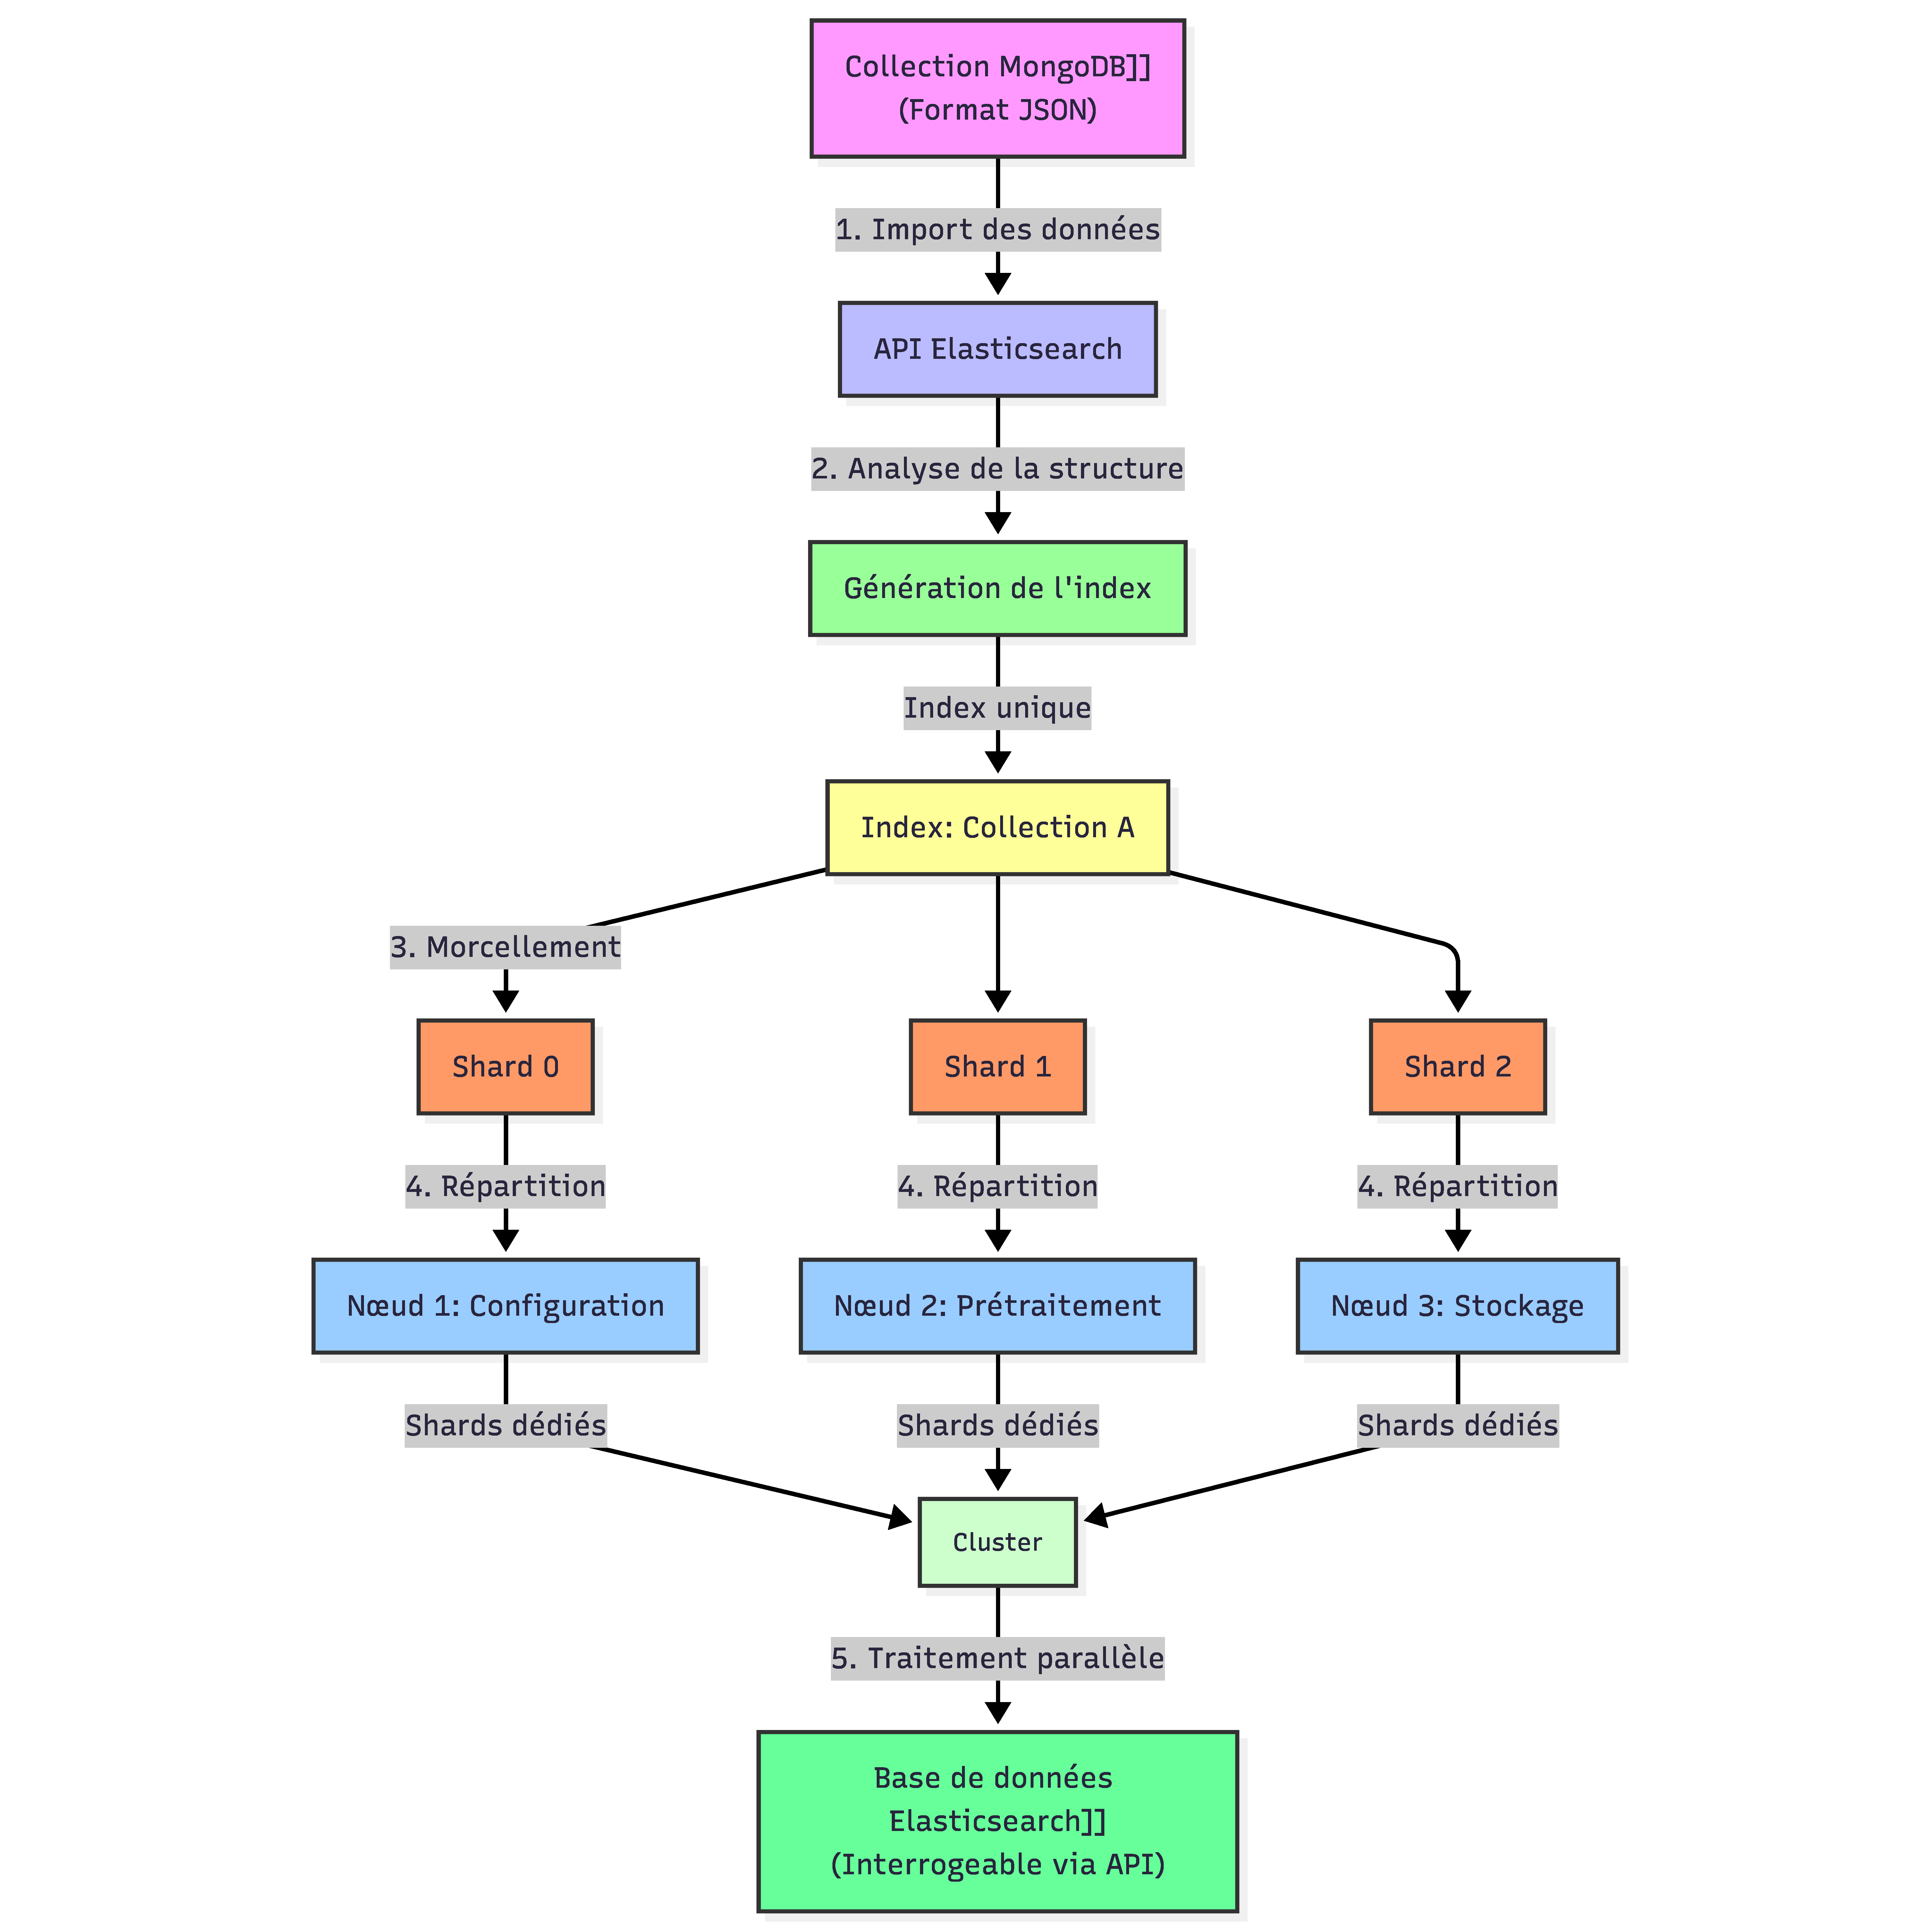
\includegraphics[width=0.8\textwidth]{./Schema/ElasticSearch.pdf}
	\caption{Schéma du fonctionnement d'Elasticsearch }
	\label{fig:elasticsearch_schema}
\end{figure}

\newpage

Ce système est donc lié à l'applicatif : il n'est pas un composant créé par l'application mais bien un élément externe relié à l'application. ElasticSearch propose ses propres modalités de recherche : recherche simple, recherche full-text\footnote{méthode de recherche qui explore des documents entiers à la recherche de chaîne de caractères demandées.}, recherche par mots-clés, recherche avancée ou bien par facettes, disons par catégorie et récurrence des données. Pour faciliter l'usage, l'application à créer une barre de recherche qui permet à l'utilisateur de créer ces requêtes de manière visuelle et interactive. C'est une interface \textit{no-code} qui permet d'envoyer les requêtes depuis l'application vers l'API ElasticSearch.\newline

\label{limites-SRI}Cependant, ces \gls{SRI} comme ElasticSearch rencontrent des limites dans l'exploitation des données des institutions patrimoniales. En effet,leurs structures ce sont largement complexifiées : d'abord par l'arrivée de nouvelles normes, modifiant des structures, et ensuite par le phénomène de densification des bases de données rendant leurs interrogation plus difficiles. Ces éléments n'ont fait que de mettre en évidences des limites déjà présentes, mais qui n'était pas forcément bloquantes. 

D'abord, ces systèmes ne prennent pas en compte la notion de contexte. La recherche s'effectue sur des critères de pertinences attribués par la correspondance de mots-clés. Ces mots clés sortent deux informations de leurs contextes : d'abord le mot qui peut avoir plusieurs significations en fonction du document et de la phrase, son contexte. Ainsi on risque d'avoir des résultats manquants de pertinence puisque la sémantique n'est pas intégrée. Ensuite, un document peut avoir un tout autre sens lorsqu'il est liés à un ensemble de documents. Or, l'analyse par mots-clés ne prend pas en compte cette notion. Ainsi, une recherche renverra vers une pièce d'archive d'un fonds mais pas vers les autres composants de ce même fonds. Seule la pièce pertinente sera renvoyée à l'utilisateur sans le fonds auquel il se rattache ce qui peut être bloquant pour un chercheur.

De plus, le système de correspondance par mots-clés des \gls{SRI} est fragile face aux variations d'indexation. Malgré les efforts de normalisation qui ont été menés, l'indexation humaine est par nature variable. Deux personnes vont décrire un même objet en utilisant des mots différents et le principe de correspondance par mots-clés est trop sensible à cette variabilités.\footcite[p.273]{koolenInformationRetrievalCultural2013} ElasticSearch, par exemple, s'appuie sur le modèle BM25 qui établi la pertinence en se basant sur la fréquence des termes. Il est donc en proie à deux limites : l'utilisations de même terme pour définir des réalités différentes d'une part, et leurs utilisations dans des contextes différents d'autres parts. Cela brouille les capacités d'analyses du logiciel ce qui impact la qualité et l'exhaustivité des résultats. En effet, un document présentant une fréquence de terme "pertinents" moins hautes qu'un autre ne signifie pas qu'il est moins pertinent. Le \gls{SRI} n'intègrent pas cette notion et propose donc des résultats parfois non pertinents. 
Cette limite peut être élargie au contenus même des documents historiques, de plus en plus renseignés dans les bases de données grâces aux technologies d'\gls{OCR} et d'\gls{HTR}. Le vocabulaire employé provoque une double difficulté : la correspondance sémantique et terminologique avec le langage actuel, et la variation de l'écriture d'un même mot à travers le temps. Les \gls{SRI} n'associent pas les termes historiques à des équivalents actuels ou à leurs évolutions orthographiques. Certaines recherches peuvent alors manquer d'outil précis.\footcite[]{ranjgarCulturalHeritageInformation2024} \label{Keyword}

Ensuite, ces systèmes sélectionnent les données pertinentes par proximité thématique. C'est à dire que des données se rattachant à des thèmes similaires sont retournées à l'utilisateur ensemble. Dans le domaine patrimoniale, des proximités thématique existent entre des typologies documentaires différentes, ce que les \gls{SRI} n'exploite pas puisqu'ils cloisonnent ces dernières.\footcite{koolenInformationRetrievalCultural2013}.\newline


Une autre difficulté est celle du cloisonnement terminologique des typologies patrimoniales. L'hétérogénéité des collections est prise en charge par la plus part des applications. SkinSoft le fait également à travers ces modules dédiés à chaque typologie\footnote{Voir page \ref{module}}. C'est ce qu'on appelle le traitement par silo : chaque typologie documentaire ayant son propre silo, schéma d'indexation et vocabulaire. Ainsi, les \gls{SRI} ont du mal à établir une porosité entre les silos ce qui ne reflète pas la réalité scientifique puisque des connexions sémantiques existent.\footcite[p.274]{koolenInformationRetrievalCultural2013} Pour le logiciel SkinSoft, cette limite est à nuancer : un outil de "recherche fédérée" permet de faire des correspondances entre ces silos. Ainsi, il est possible de rechercher à travers toutes les typologies documentaires via des correspondances de champs. Cependant, il y a des limites : seules certaines typologies documentaires sont interrogeable et uniquement sur un nombre restreint de champs. Car si des correspondances existent, elles ne sont pour autant pas évidente à traduire dans un \gls{SRI} qui est trop rigide.\newline
	
De plus, il y a un décalage entre croissant entre les pratiques des utilisateurs et les outils proposés par ces systèmes. Ce n'est que très récemment que des études ont été menées sur ce sujet\footcite{warwickIfYouBuild2007} et elles révèlent 3 problèmes fondamentaux : 
\begin{enumerate}
	\item D'abord, l'amélioration des navigateurs en lignes, tels Google, ont habitué l'utilisateur a fonctionner par échantillonage : la pertinence des résultats est analysée à partir de quelques pages seulement. Ainsi, quand les \gls{SRI} génèrent du bruit, il y a un désintérêt utilisateurs pour les résultats retournés.\footcite[p.9]{warwickIfYouBuild2007}
		
	\item \label{modalités-recherches} Ensuite, la complexité des interfaces de recherches. En effet, les utilisateurs n'ont pas l'habitude d'utiliser la recherche avancée, la recherche fédérée, les facettes, la recherche plein texte ciblée ou bien encore la recherche croisée propres aux \gls{SRI}. C'est une interface simple, qui renvoie des résultats pertinents et qui est donc bien plus attractive. Ainsi, aux yeux d'utilisateur ses outils perdent en intérêt et en praticité.\footcite[p.23-24]{warwickIfYouBuild2007}
		
	\item Enfin les \gls{SRI} ont leurs propres manière de structurer et indexer les données. Cela impacte directement la qualité des résultats retournés. Ces éléments sont cependant opaque, ce qui freine les chercheurs, notamment, à accorder une confiance complète aux résultats retournés. \label{opaque}
\end{enumerate} 
	
D'une manière plus générale, un utilisateur en face d'un outil opaque, proposant une interface complexe et des résultats bruités risque d'accorder moins de crédits au logiciel et s'en désintéresser.
	
Nous devons quand même nuancer ce propos. L'étude mentionnée traite des réactions et habitudes d'utilisateurs en tout genre face aux interfaces des sites d'institutions culturelles. Ce n'est pas une étude de comportement de professionnel face à des \terme{SGC}. 

Ainsi, l'impact des 3 points relevés n'est pas équivalents à ce qui est mentionné dans notre cas. Il est cependant une réalité que nos habitude d'utilisateur de moteur de recherche comme Google influence nos habitudes et attentes professionnelles. Au cours du stage, quelques retours utilisateurs m'ont permis d'associer les difficultés reportés dans l'article mentionné aux difficultées soulevées par des utilisateurs. C'est pour cette raison que figure ici ces limites, bien qu'ils soient nécessaire de les recontexualiser et de leurs accorder une moindre importance.\newline
	
Finalement, dans des collections toujours plus vastes et complexe, les \gls{SRI} ont de plus en plus de difficultés à satisfaire les exigences utilisateurs et scientifiques. La démocratisation des moteurs de recherches et des outils d'\gls{IA} changent drastiquement notre rapport à la recherche de données. Nos attentes et pratiques en mutation ont forcément un impact sur notre perception de ces outils, notre utilisations de ces derniers et donc leurs évolutions. 
	
C'est particulièrement visible dans l'outil SkinSoft reposant sur une base de donnée No-SQL de plusieurs dizaines de \gls{col} et aux données très variées. L'utilisation d'une indexation par mots-clés traditionnelles offre des performances limitées : on obtient facilement beaucoup de bruit à moins de savoircomment retrouver ce que l'on cherche. L'une des causes est la répétition des \gls{chps} dans l'application : un même champs peut apparaître plusieurs fois et contenir des données de nature différentes. De plus, SkinSoft propose son logiciel afin de gérer tous les types de collections : des plus petites et homogènes, aux plus vastes et hétérogènes. Plus la collections est vaste et hétérogène, plus le \gls{SRI} atteint ses limites et offre des performances moindre. 
	
L'\gls{SRI} est également mal adapté au principe de recherche fédérée. En effet, chaque typologie de collections est sujette à son propre module de gestion qui coexiste avec les autres. SkinSoft tire partie de cela par la recherche fédérée des modules permettant d'interroger plusieurs typologie de collections à l'aide des mêmes champs. Cependant, seulement quelques champs sont pris en comptes et le manque de compréhension contextuelle et syntaxique du \gls{SRI} est une grande limite.  
	
Ainsi, le logiciel SkinSoft cherche à améliorer son système de recherche par le \gls{NLP} afin de réduire le bruit généré, développer sa recherche fédérée, répondre à des requêtes plus exigeantes tout en offrant une plus grande simplicité d'usage. De plus, cela permettrais d'harmoniser les performances offertes par le moteur de recherche puisque cela permettrais de traiter plus facilement de plus grands jeux de données.\newline
	
Pour l'axe de l'amélioration de l'usage applicatif, nous nous retrouvons dans un domaine moins exploré. Deux éléments sont centraux : le premier est l'amélioration de l'usage utilisateur de l'application et de la compréhension qu'il en a. C'est à dire qu'on envisage le \gls{NLP}, notamment à travers un \gls{ac}, comme un moyen guider l'utilisateur au sein de l'application. Le second est de proposer un appui à la production de données patrimoniales propres et interopérables, toujours à travers un \gls{ac}. Il pourrait vérifier la saisie des métas données et les contradictions potentielles d'ordre sémantique. Ou encore les contradictions avec des normes descriptives appliquées aux domaines documentaires dans lequel on se trouve. Commençons par le premier point : 
	
L'agent conversationnel, comme ChatGPT, connaît une dyanmique de croissance technologique et de diffusion très importantes ces dernières années. L'outil se fait remarquer par sa capacité d'interraction avec un utilisateur par l'usage du \gls{NLP}. Cette caractéristique a tout de suite été vu comme l'opportunité de faire parler les collections et de faciliter les parcours utilisateurs sur les portails institutionnel. Plusieurs initiatives ont visées à concrétiser cette opportunité, comme celle des musées d'histoire naturelle Australien.\footcite{wangConversationalAIEnhancedExploration2026} 
	
Ces études ont amené à réfléchir sur les interfaces métier des \terme{SGC}. Il y a un véritable questionnement naissant sur l'impact des interfaces proposées dans les \guillemetleft logiciels métiers \guillemetright \footnote{Logiciel conçu pour répondre à des besoin professionnels.} \space sur la gestion des collections. 
	
Ces études abordent notamment la \guillemetleft surcharge cognitive \guillemetright \space, \label{cognitif} c'est à dire quand une interface propose trop d'informations et d'interractions différentes au point de perdre l'utilisateur.\footcite[p.1-4]{paasCognitiveLoadTheory2010}. Dans un \terme{SGC}, la principale source de surcharge cognitive est l'interactivité des éléments. En effet, un objet est reliés à énormément d'éléments individuel mais constamment en lien. Dès lors, la multiplicitées de ces connexions et leurs complexités peut surcharger l'utilisateur et conduire à faire des erreurs. Cela peut également créer une charge mentale encombrante pour l'utilisateur réduisant sa concentration.\footcite[p.2]{paasCognitiveLoadTheory2010} Cela relève de ce qu'on appel l'\gls{ux}, c'est à dire la manière de simplifier l'expérience utilisateur.
	
Le second point est celui de l'interface en elle même. L'interface reflète bien souvent la complexité logicielle et perd l'utilisateur dans son usage applicatif. La multiplications des points d'entrées par exemple dénue l'application de repère visuelle et exige une expérience de l'application. \footcite[p.153]{nielsenEnhancingExplanatoryPower1994} Plus important encore, l'interface est importante pour la gestion de l'information. Quand trop d'options ou d'actions sont proposées, l'informations essentielles à extraire ou intégrer échappe à l'utilisateur. Cela peut pousser un utilisateur à éviter ces endroits surchargés et donc ne pas utiliser certaines fonctionnalitées \footcite[p.153-154]{nielsenEnhancingExplanatoryPower1994}. Tout cela relève de ce qu'on appelle aujourd'hui l'\gls{ui}, où la manière de créer des interfaces logicielles pratiques et simples.
	
Le logiciel SkinSoft se heurte à certaines de ses complexités. Prenons les points d'accès : bien que groupés à un même endroit dans l'applicatif ils sont nombreux et produise un effet de masse. C'est le propre des logiciels de \terme{SGC} car la gestion d'un tel spectre de données mutliplient nécessairement les point d'accès. La simplifications de l'interface ne peut effacer cette première complexité car l'accès à chacun de ces points d'entrées est nécessaire. De plus, les interractions entre ces éléments sont nombreuses et demandent différentes fonctionnalités situées à différents endroits. C'est encore une fois le propre des \terme{SGC} : prenons l'objets, il reste au c\oe{ur} d'un bon nombre d'éléments ce qui fait de lui un n\oe{ud} central. Ainsi, il multiplie les points d'accès et les fonctionnalités associées : depuis un objet on peu créer un ensemble, un projet, une entrée, une sortie, un prêt, et bon nombre d'éléments.

Un autre problème rarement cités dans les études est la duplication de documentation externe. En effet, les fournisseurs logiciels produisent de la documentation métier destinées à guider l'utilisateur. Cependant, cette document n'est pas dans l'application : elle se trouve dans un dépôt externe. Ainsi, quand un utilisateur recontre une difficultés, il doit ressort de l'application afin de consulter un manuel, ou plusieurs. L'accessibilité à l'informations est un véritable problème : une réponse complexe à trouvée entraîne la perte d'intérêt.
	
Si des chercheurs proposent de décharger les interfaces afin de les rendres intuitives\footcite{whitelawGenerousInterfacesDigital2015}, l'ampleur de la tâche dans les \terme{SGC} est telle qu'on envisage de nouvelles solutions. Le logiciel SkinSoft le démontre bien : l'interface épurée, les efforts de regroupement d'éléments et de leurs répartitions ne suffisent pas à pallier la complexité native dû au \terme{SGC}. L'émergence des agents conversationnel ouvre une nouvelle possibilité : interagir avec l'application par de simple requête. De cette manière, il peut disposer d'un guide interactif qui a la capacité de s'appuyer sur cette documentation métier externe. Cet agent conversationnel peut d'ailleurs être le socle d'une technologie plus importante qu'est celle de l'agent IA, qui est capable lui d'interragir avec l'application.\newline
	
Pour le second point, très peu d'articles, pour ne pas dire presque aucun, ont été produit sur le sujet. Beaucoup énonce l'idée de faire de l'agent conversationnel un assitant de production, mais très peux y apporte une véritable dimension académique ou des propositions d'implémentation. C'est donc une partie bien plus théorique et expérimentale qui est abordée dans ce point. 
	
Des interfaces trop riches peuvent favoriser la saisie d'erreur dans les métas données, ce qui finit par constituer une bases de données instable. Mais ce n'est pas la seule explication : la redondance de la tâche ainsi que la difficulté à renseigner certains objets en sont des explications plus importantes encore. 
	
Ainsi, sur de large jeux de données, toujours en expansion, les moyens de contrôle actuels mis en place, comme des formulaires de saisies et des champs contrôlés, sont de plus en plus limitées.\footcite[p.2]{lewisImpactHumanDecisionMaking2025} En effet, plus la quantité de données à traiter est importante, plus la fiabilité humaine laisse place à des oublis, des erreurs de saisies et des incohérences de données. Si les erreurs sont très nombreuses et variées, les résulats lors du requêtage perdent en qualité\footcite[p.4]{lewisImpactHumanDecisionMaking2025}.
	
De plus, certaines collections spécifiques demandent des traitements particuliers. Prenons l'exemple des collections d'histoire naturelle, notamment des spécimens qui sont nombreux et centraux dans ces collections. Ils se rattachent à des classifications taxonomiques qui ne sont pas fixes : souvent hypothètiques, elles sont ensuite remaniées ou invalidées. Ces changements sont fréquents et concerne assez rapidement un grand nombre de specimens et donc de notice dans un \terme{SGC}. Il est donc souvent impossible d'assurer la mise à jour totale des espèces dans les grandes bases de données\footcite{hedrickDigitizationFutureNatural2020} Ainsi, un agent conversationnel capable de signaler à l'utilisateur la nécessité de mettre à jour certaines notices est particulièrement pertinent. Un agent IA capable de le faire seul, l'est d'autant plus.\newline
	
Le logiciel SkinSoft est un bon exemple des difficultées actuelles rencontrées par les \terme{SGC} et les limites des solutions déjà existantes. En effet, la simplification de l'interface et de l'expérience utilisateurs par l'application des principes d'\gls{ui} et d'\gls{ux} est limitées. La complexité native de ces systèmes ne peut être résolue entièrement de cette manière. La massification des données et l'hétérogénéité typologiques des collections constituent des défis demandant de nouveaux moyens de réponses. Ce manque de solutions est dû à un changement de problématique : la question n'est plus de faciliter, mais de créer de nouveaux outils pour combler l'écart entre la capacité de traitement humaine insuffisante face aux besoins du traitement des données massives et hétérogènes.
		
Ainsi, on comprends que l'intégration d'un agent conversationnel dans l'application a deux enjeux. Le premier enjeux est de simplifier la circulation et l'utilisation de l'application dans sa globalité. Cela est envisagé par la possibilité de converser avec un assistant spécialisé capable de guider en s'appuyant sur de la documentation métier contrôlée. Le second enjeux est donc de disposer d'un assistant capable de tracer l'activité faite, celle à faire et ainsi que la qualité de ce qui est déjà présent. De cette manière, il va pouvoir apporter une solution au problème principal que tout changement d'interface ne peut régler : la faillibilité humaine.
	
Le \gls{NLP} semble aujourd'hui apporté des éléments de réponses afin de combler cet écart. La capacité de cette technologie à interragir avec l'utilisateur et à comprendre les données à une échelle massive ouvre de nouvelles possibilités d'usages et d'interfaces qui permettrait de résoudres les problématiques relatives aux \terme{SGC}. Cependant, cette technologie recouvre un ensemble vaste d'outils et de réalités techniques\footnote{ Voir page \pageref{1.2.1}}, ce qui demande de les séparer en deux outils différents : la recherche augmentée, répondant aux problématique soulevées dans le premier point, et un \guillemet{chatbot}, répondant aux problématiques soulevées dans le second point.
	
	
	
	
	
	
